\documentclass{standalone}
\usepackage{tikz}
\usetikzlibrary{patterns, positioning}
\usepackage[sfdefault]{ClearSans} %% option 'sfdefault' activates Clear Sans as the default text font
\usepackage[T1]{fontenc}

\begin{document}
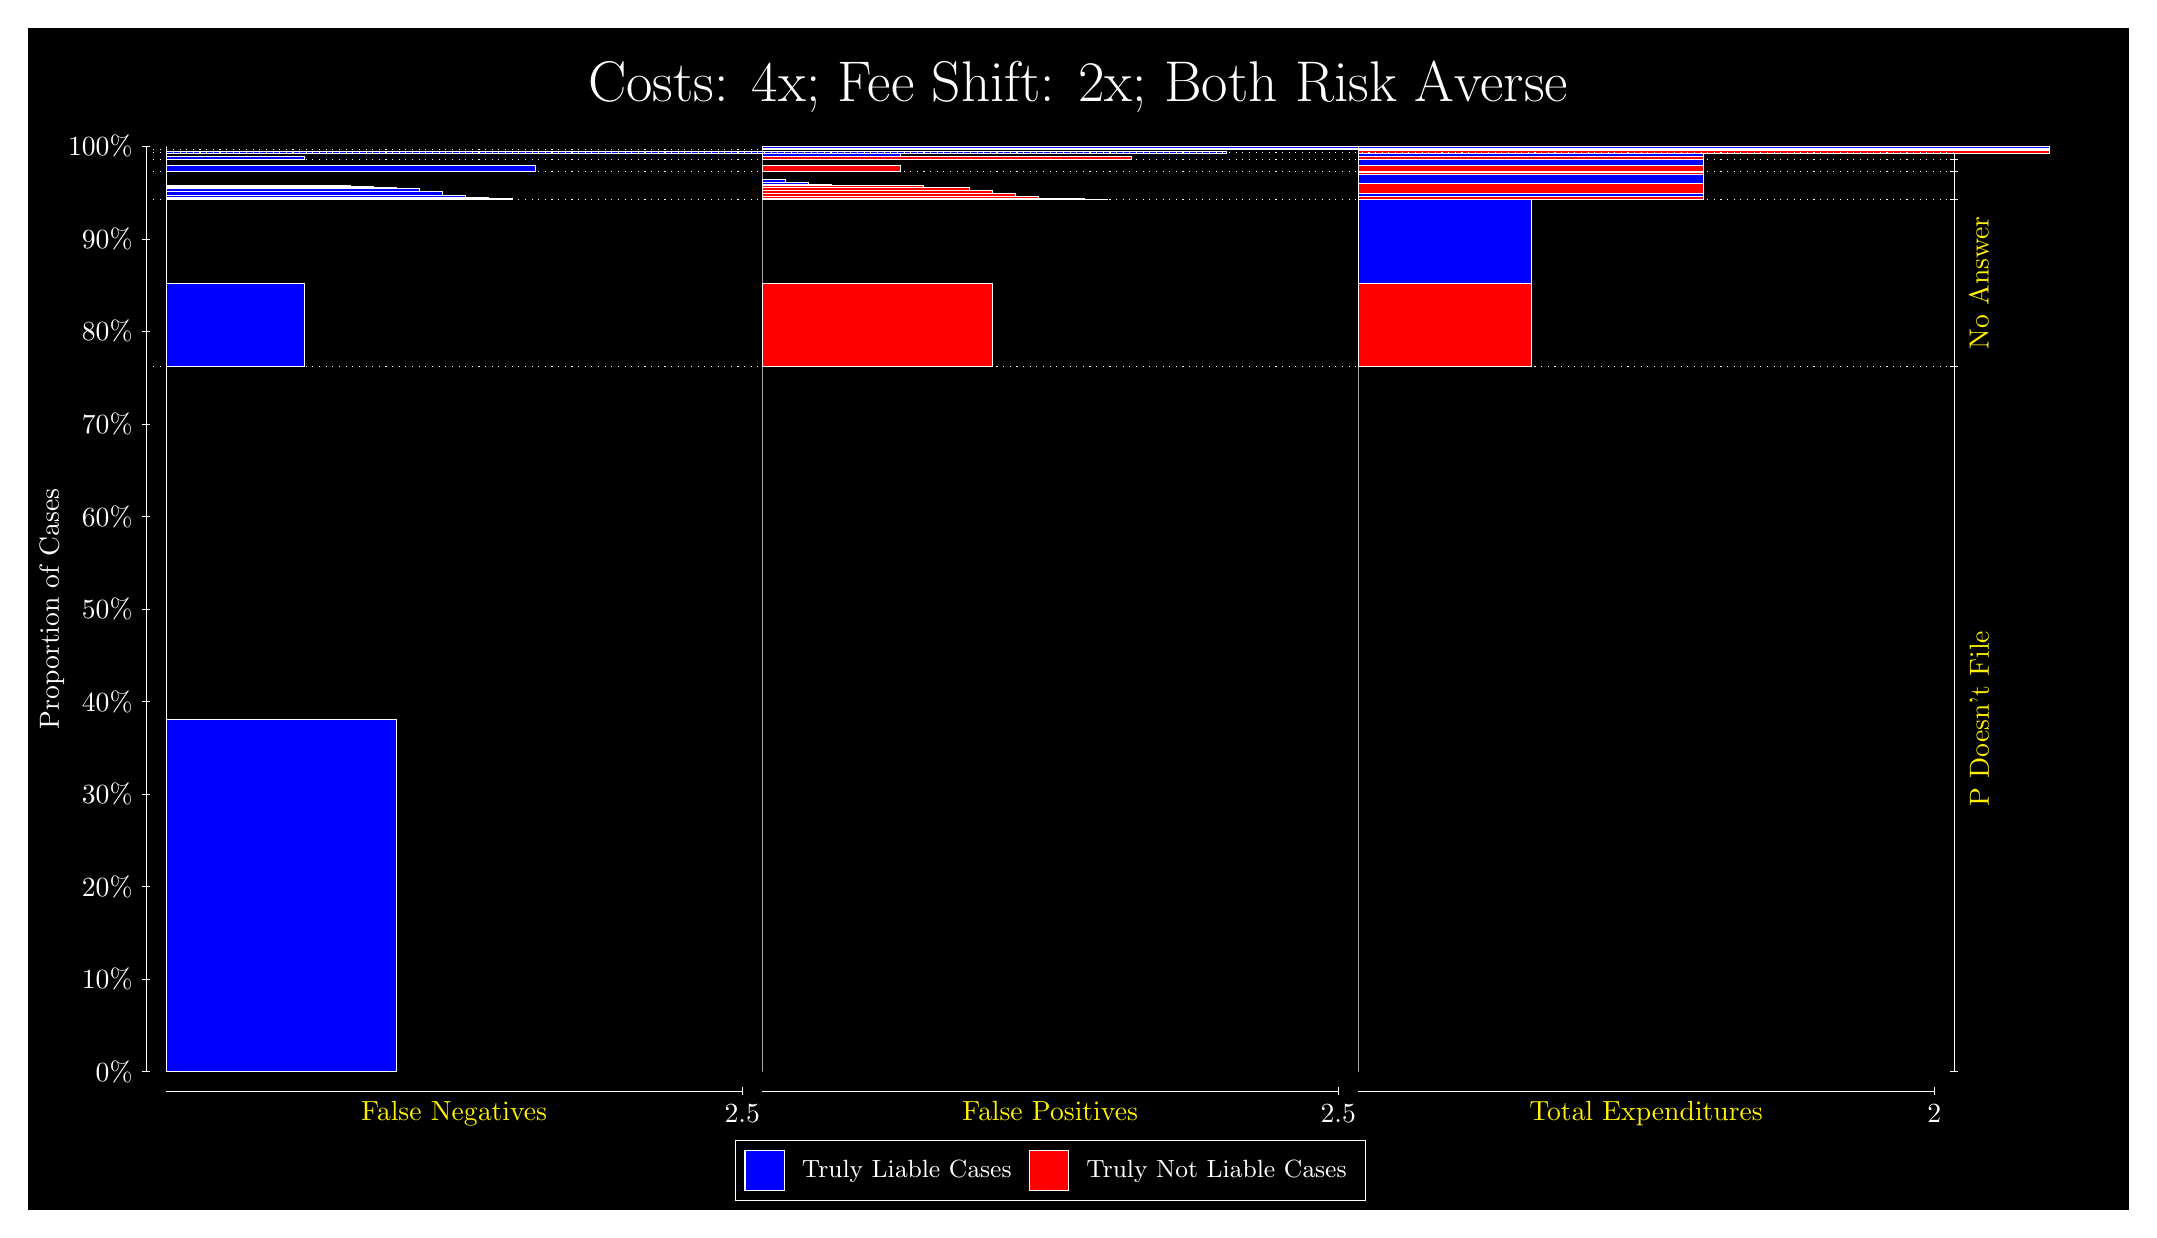
\begin{tikzpicture}
\draw[fill=black] (0,0) rectangle (26.667,15);
\draw[text=white] (0,13.5) rectangle (26.667,15) node[midway] {\huge Costs: 4x; Fee Shift: 2x; Both Risk Averse};
\draw[white, very thin] (1.5,1.75) -- (1.5,13.5);
\node[rotate=90, text=white, anchor=center] at (0.3, 7.625) {Proportion of Cases};
\draw[white, very thin] (1.45,1.75) -- (1.55,1.75);
\node[text=white, anchor=east] at (1.45, 1.75) {0\%};
\draw[white, very thin] (1.45,2.925) -- (1.55,2.925);
\node[text=white, anchor=east] at (1.45, 2.925) {10\%};
\draw[white, very thin] (1.45,4.1) -- (1.55,4.1);
\node[text=white, anchor=east] at (1.45, 4.1) {20\%};
\draw[white, very thin] (1.45,5.275) -- (1.55,5.275);
\node[text=white, anchor=east] at (1.45, 5.275) {30\%};
\draw[white, very thin] (1.45,6.45) -- (1.55,6.45);
\node[text=white, anchor=east] at (1.45, 6.45) {40\%};
\draw[white, very thin] (1.45,7.625) -- (1.55,7.625);
\node[text=white, anchor=east] at (1.45, 7.625) {50\%};
\draw[white, very thin] (1.45,8.8) -- (1.55,8.8);
\node[text=white, anchor=east] at (1.45, 8.8) {60\%};
\draw[white, very thin] (1.45,9.975) -- (1.55,9.975);
\node[text=white, anchor=east] at (1.45, 9.975) {70\%};
\draw[white, very thin] (1.45,11.15) -- (1.55,11.15);
\node[text=white, anchor=east] at (1.45, 11.15) {80\%};
\draw[white, very thin] (1.45,12.325) -- (1.55,12.325);
\node[text=white, anchor=east] at (1.45, 12.325) {90\%};
\draw[white, very thin] (1.45,13.5) -- (1.55,13.5);
\node[text=white, anchor=east] at (1.45, 13.5) {100\%};

\draw[white, very thin] (24.457,1.75) -- (24.457,13.5);
\draw[white, very thin] (24.407,1.75) -- (24.507,1.75);
\node[anchor=west] at (24.407, 1.75) {};
\draw[white, very thin] (24.407,10.709) -- (24.507,10.709);
\node[anchor=west] at (24.407, 10.709) {};
\draw[white, very thin] (24.407,12.824) -- (24.507,12.824);
\node[anchor=west] at (24.407, 12.824) {};
\draw[white, very thin] (24.407,13.183) -- (24.507,13.183);
\node[anchor=west] at (24.407, 13.183) {};
\draw[white, very thin] (24.407,13.332) -- (24.507,13.332);
\node[anchor=west] at (24.407, 13.332) {};
\draw[white, very thin] (24.407,13.418) -- (24.507,13.418);
\node[anchor=west] at (24.407, 13.418) {};
\draw[white, very thin] (24.407,13.459) -- (24.507,13.459);
\node[anchor=west] at (24.407, 13.459) {};
\draw[white, very thin] (24.407,13.5) -- (24.507,13.5);
\node[anchor=west] at (24.407, 13.5) {};

\draw[white, very thin, fill=blue] (1.75,1.75) rectangle (4.6775,6.2294);
\draw[white, very thin, fill=red] (1.75,6.2294) rectangle (1.75,10.709);
\draw[white, very thin, fill=blue] (1.75,10.709) rectangle (3.5065,11.765);
\draw[white, very thin, fill=red] (1.75,11.765) rectangle (1.75,12.824);
\draw[white, very thin, fill=blue] (1.75,12.824) rectangle (6.1413,12.839);
\draw[white, very thin, fill=blue] (1.75,12.839) rectangle (5.8486,12.848);
\draw[white, very thin, fill=blue] (1.75,12.848) rectangle (5.5558,12.884);
\draw[white, very thin, fill=blue] (1.75,12.884) rectangle (5.2631,12.927);
\draw[white, very thin, fill=blue] (1.75,12.927) rectangle (4.9703,12.967);
\draw[white, very thin, fill=blue] (1.75,12.967) rectangle (4.6775,12.984);
\draw[white, very thin, fill=blue] (1.75,12.984) rectangle (4.3848,12.995);
\draw[white, very thin, fill=blue] (1.75,12.995) rectangle (4.092,13.001);
\draw[white, very thin, fill=blue] (1.75,13.001) rectangle (3.7993,13.006);
\draw[white, very thin, fill=red] (1.75,13.006) rectangle (1.75,13.183);
\draw[white, very thin, fill=blue] (1.75,13.183) rectangle (6.4341,13.256);
\draw[white, very thin, fill=red] (1.75,13.256) rectangle (1.75,13.332);
\draw[white, very thin, fill=blue] (1.75,13.332) rectangle (3.5065,13.376);
\draw[white, very thin, fill=red] (1.75,13.376) rectangle (1.75,13.418);
\draw[white, very thin, fill=blue] (1.75,13.418) rectangle (15.217,13.433);
\draw[white, very thin, fill=red] (1.75,13.433) rectangle (1.75,13.459);
\draw[white, very thin, fill=red] (1.75,13.459) rectangle (1.75,13.475);
\draw[white, very thin, fill=blue] (1.75,13.475) rectangle (1.75,13.5);
\draw[white, very thin, fill=red] (9.3189,1.75) rectangle (9.3189,6.2294);
\draw[white, very thin, fill=blue] (9.3189,6.2294) rectangle (9.3189,10.709);
\draw[white, very thin, fill=red] (9.3189,10.709) rectangle (12.246,11.767);
\draw[white, very thin, fill=blue] (9.3189,11.767) rectangle (9.3189,12.824);
\draw[white, very thin, fill=red] (9.3189,12.824) rectangle (13.71,12.829);
\draw[white, very thin, fill=red] (9.3189,12.829) rectangle (13.417,12.834);
\draw[white, very thin, fill=red] (9.3189,12.834) rectangle (13.125,12.846);
\draw[white, very thin, fill=red] (9.3189,12.846) rectangle (12.832,12.862);
\draw[white, very thin, fill=red] (9.3189,12.862) rectangle (12.539,12.901);
\draw[white, very thin, fill=red] (9.3189,12.901) rectangle (12.246,12.941);
\draw[white, very thin, fill=red] (9.3189,12.941) rectangle (11.954,12.976);
\draw[white, very thin, fill=red] (9.3189,12.976) rectangle (11.661,12.985);
\draw[white, very thin, fill=red] (9.3189,12.985) rectangle (11.368,13.001);
\draw[white, very thin, fill=blue] (9.3189,13.001) rectangle (10.783,13.006);
\draw[white, very thin, fill=blue] (9.3189,13.006) rectangle (10.49,13.011);
\draw[white, very thin, fill=blue] (9.3189,13.011) rectangle (10.197,13.023);
\draw[white, very thin, fill=blue] (9.3189,13.023) rectangle (9.9044,13.04);
\draw[white, very thin, fill=blue] (9.3189,13.04) rectangle (9.6116,13.08);
\draw[white, very thin, fill=blue] (9.3189,13.08) rectangle (9.3189,13.183);
\draw[white, very thin, fill=red] (9.3189,13.183) rectangle (11.075,13.259);
\draw[white, very thin, fill=blue] (9.3189,13.259) rectangle (9.3189,13.332);
\draw[white, very thin, fill=red] (9.3189,13.332) rectangle (14.003,13.374);
\draw[white, very thin, fill=blue] (9.3189,13.374) rectangle (11.075,13.418);
\draw[white, very thin, fill=red] (9.3189,13.418) rectangle (9.3189,13.445);
\draw[white, very thin, fill=blue] (9.3189,13.445) rectangle (9.3189,13.459);
\draw[white, very thin, fill=red] (9.3189,13.459) rectangle (22.786,13.475);
\draw[white, very thin, fill=blue] (9.3189,13.475) rectangle (19.858,13.5);
\draw[white, very thin, fill=red] (16.888,1.75) rectangle (16.888,6.2294);
\draw[white, very thin, fill=blue] (16.888,6.2294) rectangle (16.888,10.709);
\draw[white, very thin, fill=red] (16.888,10.709) rectangle (19.083,11.767);
\draw[white, very thin, fill=blue] (16.888,11.767) rectangle (19.083,12.824);
\draw[white, very thin, fill=red] (16.888,12.824) rectangle (21.279,12.863);
\draw[white, very thin, fill=blue] (16.888,12.863) rectangle (21.279,12.903);
\draw[white, very thin, fill=red] (16.888,12.903) rectangle (21.279,13.025);
\draw[white, very thin, fill=blue] (16.888,13.025) rectangle (21.279,13.149);
\draw[white, very thin, fill=red] (16.888,13.149) rectangle (21.279,13.166);
\draw[white, very thin, fill=blue] (16.888,13.166) rectangle (21.279,13.183);
\draw[white, very thin, fill=red] (16.888,13.183) rectangle (21.279,13.259);
\draw[white, very thin, fill=blue] (16.888,13.259) rectangle (21.279,13.332);
\draw[white, very thin, fill=red] (16.888,13.332) rectangle (21.279,13.374);
\draw[white, very thin, fill=blue] (16.888,13.374) rectangle (21.279,13.418);
\draw[white, very thin, fill=red] (16.888,13.418) rectangle (25.67,13.445);
\draw[white, very thin, fill=blue] (16.888,13.445) rectangle (25.67,13.459);
\draw[white, very thin, fill=red] (16.888,13.459) rectangle (25.67,13.475);
\draw[white, very thin, fill=blue] (16.888,13.475) rectangle (25.67,13.5);
\draw[white, dotted] (1.5,10.709) -- (24.457,10.709);
\draw[white, dotted] (1.5,12.824) -- (24.457,12.824);
\draw[white, dotted] (1.5,13.183) -- (24.457,13.183);
\draw[white, dotted] (1.5,13.332) -- (24.457,13.332);
\draw[white, dotted] (1.5,13.418) -- (24.457,13.418);
\draw[white, dotted] (1.5,13.459) -- (24.457,13.459);
\draw[white, very thin] (1.75,1.5) -- (9.0689,1.5);
\node[text=yellow, anchor=north] at (5.4094, 1.5) {False Negatives};
\draw[white, very thin] (9.0689,1.45) -- (9.0689,1.55);
\node[text=white, anchor=north] at (9.0689, 1.45) {2.5};

\draw[white, very thin] (9.3189,1.5) -- (16.638,1.5);
\node[text=yellow, anchor=north] at (12.978, 1.5) {False Positives};
\draw[white, very thin] (16.638,1.45) -- (16.638,1.55);
\node[text=white, anchor=north] at (16.638, 1.45) {2.5};

\draw[white, very thin] (16.888,1.5) -- (24.207,1.5);
\node[text=yellow, anchor=north] at (20.547, 1.5) {Total Expenditures};
\draw[white, very thin] (24.207,1.45) -- (24.207,1.55);
\node[text=white, anchor=north] at (24.207, 1.45) {2};

\node[text=yellow, centered, rotate=90] at (24.777, 6.2294) {P Doesn't File};
\node[text=yellow, centered, rotate=90] at (24.777, 11.766) {No Answer};






\draw (12.978300999999998,1.5) node[draw=none] (baseCoordinate) {};
\begin{scope}[align=center]
        \matrix[scale=0.5, draw=white, below=0.5cm of baseCoordinate, nodes={draw}, column sep=0.1cm]{
            \node[rectangle, draw, minimum width=0.5cm, minimum height=0.5cm, fill=blue] {}; &
            \node[draw=none, font=\small, text=white] (B) {Truly Liable Cases}; &
            \node[rectangle, draw, minimum width=0.5cm, minimum height=0.5cm, fill=red] {}; &
            \node[draw=none, font=\small, text=white] (B) {Truly Not Liable Cases}; \\
            };
\end{scope}

\end{tikzpicture}
\end{document}